\chapter{A Different Way Of Living}

This chapter follows J. Krishnamurti's dialogue with Alan W. Anderson as an inquiry into living, love, death, and consciousness. There are no blackboard equations in this lecture. The mathematical structure here is therefore not a physics derivation but a disciplined map of distinctions: conflict and perception, fragmentation and wholeness, continuity and immediate action. We will use compact notation only where it helps us keep the inquiry precise.

\section{The Question Resumed: Living, Love, Death}

The dialogue begins by taking up an unfinished question. Anderson recalls that the previous conversation had begun to look at the relation among living, love, and death. Krishnamurti does not begin with death as a doctrine or with love as an ideal. He sets the order carefully. First we must ask what we actually call living.

The reason for this order is important. If ordinary living is already confused, frightened, fragmentary, and in conflict, then any answer about love or death that grows out of that confusion will carry the same disorder. So the first move is not metaphysical. It is diagnostic.

We can write the opening order as a simple sequence:
\begin{equation}
\text{living} \longrightarrow \text{love} \longrightarrow \text{death}.
\end{equation}
This is not a chronological law. It is the order of inquiry. We begin with the fact nearest to us: the way we live.

Krishnamurti's first description of living is deliberately concrete. Living is not introduced as a noble abstraction. It is work, relationship, ambition, economic pressure, frustration, holiday escape, violence, despair, and the repeated effort to become something more than what one is. The word he returns to is battle.

\section{What We Call Living}

The lecture first asks us to look at the field of ordinary existence. The same pattern appears in relationship, in business, in the religious life, in politics, in education, and in private ambition. The human being wants to be different, more successful, more secure, more fulfilled. Out of that movement comes struggle.

A compact map of this first diagnosis is:
\begin{equation}
\text{daily living}
   \longrightarrow
\{\text{struggle},\ \text{pain},\ \text{frustration},\ \text{violence},\ \text{escape}\}.
\end{equation}

The examples matter. Krishnamurti speaks of the office, the factory, the short holiday that becomes a reaction against monotony, the rush from museum to museum, the romantic escape into distant cultures or costumes. These are not decorative examples. They show that escape and conflict are not separate. The holiday can be a continuation of the same life, only in another form.

The lecture then lets Anderson state the inherited assumption: we have taken for granted that life is a battle. We ask how to fight more successfully, how to minimize strain, how to endure, how to avoid collapse. But we rarely ask whether battle is living at all.

\subsection{Question \& Answer}

\paragraph{Question.}
Must life be a battle? Is struggle simply part of existence, inherited from the animal, and therefore unavoidable?

\paragraph{Answer.}
Krishnamurti's answer is not that we should improve the battle, nor that we should retreat from it into fantasy. He asks whether it is possible to live without conflict. The question must not remain verbal. It must be lived into. The point is not to adopt a theory of peace, but to see whether a different way of living is possible in daily relationship.

This is the first major conceptual turn:
\begin{equation}
\text{How do we fight better?}
\quad \leadsto \quad
\text{Can conflict end?}
\end{equation}

The shift is small in words and large in consequence. The usual question stays inside the battlefield. Krishnamurti's question asks whether the battlefield itself is necessary.

\section{Fragmentation And The Action Of Perception}

Once conflict is placed in question, Krishnamurti looks for its structure. Conflict means division. It means the battle of opposites, the separation of you and me, we and they, nation and nation, class and class, one inward fragment against another.

The basic chain is:
\begin{equation}
\text{division}
   \longrightarrow
\text{fragmentation}
   \longrightarrow
\text{conflict}
   \longrightarrow
\text{battle}.
\end{equation}

This is the central diagnostic formula of the first half of the lecture. Fragmentation is not only social. It is inward and outward at once. A fragment assumes power and dominates the other fragments. The same pattern appears in personal ambition, political division, religious obedience, class struggle, and inward contradiction.

Krishnamurti then makes an important negative point. The answer is not to integrate the fragments. Integration still begins with fragments as the given pieces and asks how to assemble them. The lecture instead turns toward perception.

\begin{definition}
In this chapter, \emph{perception} means the direct seeing of what is taking place, without a separate observer trying to change, adjust, justify, condemn, or integrate what is seen.
\end{definition}

That definition lets us write the second chain:
\begin{equation}
\text{seeing fragmentation as it is}
   \longrightarrow
\text{perception}
   \longrightarrow
\text{action}.
\end{equation}

The action that follows from perception is not an action of conflict. It is not one fragment acting on another fragment. It is not a method imposed by will. It is action born from seeing.

\subsection{A Worked Derivation: From Division To Battle}

We can state the lecture's reasoning as a short derivation. It is not a formal proof in the mathematical sense, but it has the shape of one.

\begin{enumerate}
\item Suppose living is organized around division: ``you'' and ``me,'' ``we'' and ``they,'' one class against another, one inward desire against another.
\item Division produces fragments, because each side is experienced as separate and self-protective.
\item Each fragment seeks continuity, power, or security.
\item When one fragment meets another fragment as rival or obstacle, the relation becomes conflict.
\item Repeated conflict becomes the accepted structure of living: battle.
\item Therefore, if division remains, battle is not accidental. It is built into the structure.
\end{enumerate}

In compact notation:
\begin{align}
D &:= \text{division},\\
F &:= \text{fragmentation},\\
C &:= \text{conflict},\\
B &:= \text{battle}.
\end{align}
The lecture's working chain is then:
\begin{equation}
D \longrightarrow F \longrightarrow C \longrightarrow B.
\end{equation}

The important thing is where the chain can be interrupted. Krishnamurti does not say that one fragment must defeat another. He says that the whole movement of fragmentation must be perceived.

\section{Two Energies}

The next turn comes through Anderson's question about energy. Krishnamurti has used the same word in relation to both conflict and perception, but he does not mean that the two modes are equivalent. The phenomenon is different.

Let us introduce two pieces of notation, with a caveat. These are not physical energies. They are editorial shorthand for the two modes described in the dialogue:
\begin{align}
E_{\mathrm{conflict}} &:= \text{energy released through conflict},\\
E_{\mathrm{perception}} &:= \text{energy released through perception and action}.
\end{align}

The distinction is:
\begin{align}
E_{\mathrm{conflict}}
   &\longrightarrow
   \{\text{fragmentary},\ \text{divisive},\ \text{destructive},\ \text{violent}\},\\
E_{\mathrm{perception}}
   &\longrightarrow
   \{\text{non-fragmentary},\ \text{whole},\ \text{sane},\ \text{healthy}\}.
\end{align}

Anderson gives this distinction a strong interpretive name when he speaks of the energy that shatters into fragmentary patterns as demonic. The chapter should keep this as Anderson's interpretive probe, not as a new doctrine. Krishnamurti's own emphasis is simpler: the energy of conflict is destructive; the energy of perception and action is different, non-fragmentary, and creative.

\begin{figure}
\centering
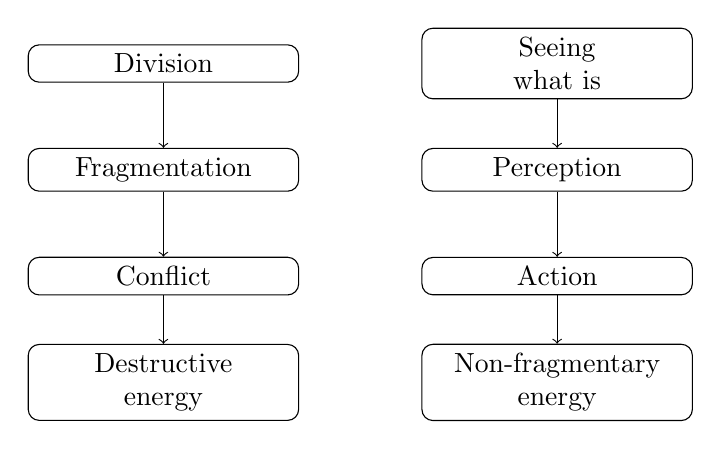
\begin{tikzpicture}[x=1cm,y=1cm]
\node[draw, rounded corners, align=center, text width=3.2cm] (d) at (0,0) {Division};
\node[draw, rounded corners, align=center, text width=3.2cm] (f) at (0,-1.35) {Fragmentation};
\node[draw, rounded corners, align=center, text width=3.2cm] (c) at (0,-2.7) {Conflict};
\node[draw, rounded corners, align=center, text width=3.2cm] (e) at (0,-4.05) {Destructive\\energy};

\node[draw, rounded corners, align=center, text width=3.2cm] (s) at (5,0) {Seeing\\what is};
\node[draw, rounded corners, align=center, text width=3.2cm] (p) at (5,-1.35) {Perception};
\node[draw, rounded corners, align=center, text width=3.2cm] (a) at (5,-2.7) {Action};
\node[draw, rounded corners, align=center, text width=3.2cm] (w) at (5,-4.05) {Non-fragmentary\\energy};

\draw[->] (d) -- (f);
\draw[->] (f) -- (c);
\draw[->] (c) -- (e);

\draw[->] (s) -- (p);
\draw[->] (p) -- (a);
\draw[->] (a) -- (w);
\end{tikzpicture}
\caption{An editorial map of the lecture's contrast between conflict and perception.}
\end{figure}

The figure should be read narrowly. It is not a formal psychological model. It is a compact way of preserving the lecture's distinction: conflict has a movement, and perception has a different movement.

\section{Education As The Test Case}

The dialogue then becomes practical. If there is a different way of living, how is it to be communicated? Anderson raises the question of education. It seems that the teacher must first be without conflict before he can teach a way of life without conflict. Krishnamurti rejects the delay hidden inside that formulation.

\subsection{Question \& Answer}

\paragraph{Question.}
Must the teacher first be transformed before teaching?

\paragraph{Answer.}
If the teacher waits until he is entirely free of conflict, he may wait forever. Krishnamurti proposes a different beginning. The teacher and the students both live in conflict. Let that fact be acknowledged. Let them look at it together in relationship. Then teaching is not the transmission of a finished authority; it is an inquiry in which both teacher and student are involved.

This gives us a simple relational update rule:
\begin{equation}
(\text{teacher in conflict},\ \text{student in conflict})
   \longrightarrow
\text{shared observation of conflict}.
\end{equation}

The point is not that technique is irrelevant in every field. Anderson explicitly worries that thought and knowledge may be misunderstood as corrupt in themselves. Krishnamurti accepts the correction: thought and knowledge have proper uses. A microphone is not corrupt. A text is not corrupt. The disorder appears when thought and knowledge become instruments of division, self-importance, authority, or escape.

So the educational example is not a detour. It is where the whole inquiry becomes testable. We do not first secure a credential of purity. We begin with the fact of conflict and look together.

\section{Love, The Field, And The End Of Separation}

Krishnamurti now returns to love. If life is battle, where can love be? If I am competing with you, trying to surpass you, using you, resisting you, or dominating you, compassion has no ground. The flame of love cannot be added to conflict as an ornament.

The lecture's compact statement is:
\begin{equation}
\text{battle} \quad \Longrightarrow \quad \text{no ground for love}.
\end{equation}

The positive statement is more subtle:
\begin{equation}
\text{perceiver} = \text{perceived}
   \quad \Longrightarrow \quad
\text{action without separation}.
\end{equation}
This formula must be handled carefully. It does not mean that ordinary objects disappear. It means that in direct perception there is no separate psychological observer standing apart from the observed and trying to manipulate it.

Anderson's example from the Gita helps the dialogue here. He speaks of the field, the classroom, and the mistake of merely telling students that there is one field. The deeper beginning is not to assert unity as a conclusion. It is to enter the field together and look.

\begin{remark}
The classroom example is crucial because it keeps the inquiry from becoming verbal. To say ``the field is one'' may still be an idea held by a lecturer. To look together in the classroom makes the classroom itself the field.
\end{remark}

This is why the lecture's movement can be summarized as:
\begin{equation}
\text{explanation of unity}
   \quad \leadsto \quad
\text{shared perception in the field}.
\end{equation}

Love, in this context, is not sentiment. It is bound up with care, responsibility, and the ending of separation in action.

\section{Consciousness, Death, And Postponement}

Only after this inquiry into living and love does Krishnamurti move toward death. He says that living, love, and death are not separate. They are one movement.

\begin{equation}
\text{living},\ \text{love},\ \text{death}
   \longrightarrow
\text{one non-divisive movement}.
\end{equation}

But he does not go straight into a doctrine of death. He first asks what consciousness is. The answer is given with deliberate simplicity:
\begin{equation}
\text{consciousness} = \text{content}.
\end{equation}
The content includes thoughts, anxieties, identifications, conflicts, attachments, fears, pleasures, agony, suffering, beliefs, and neurotic actions. We may write, cautiously:
\begin{equation}
\text{content}(\text{consciousness})
=
\{\text{thoughts},\ \text{anxieties},\ \text{identifications},\ \text{fears},\ \text{pleasures},\ \text{suffering},\ \text{beliefs}\}.
\end{equation}
This set is not exhaustive. It is a compact notation for the spoken list.

The next claim is that this content is common. My consciousness and yours may vary in detail, expansion, contraction, habit, and memory, but the structure is not essentially different. Attachment, fear, despair, belief, and the demand for continuity are not private inventions.

From this point, the question of death becomes sharper:
\begin{equation}
\text{death}
=
\begin{cases}
\text{ending of consciousness with its content},\\
\text{continuity of consciousness with its content}.
\end{cases}
\end{equation}

Krishnamurti then examines the comfort offered by belief in continuity. If I am frightened by death, someone may tell me there is life after death. I may accept reincarnation, or some equivalent promise of continuity, because I am afraid. But the belief can produce postponement. It may say: behave now, do not hurt another now. Yet if I believe there is always another chance, I may stall.

The practical chain is:
\begin{equation}
\text{belief in continuity}
   \longrightarrow
\text{comfort}
   \longrightarrow
\text{postponement}
   \longrightarrow
\text{contradiction of immediate action}.
\end{equation}

Here the word karma is kept very simple. Krishnamurti glosses it as action. He does not dwell on doctrinal complexity. The question is whether belief leads to immediate action or to delay. If it gives comfort while conduct remains unchanged, the belief has become a contradiction.

\subsection{Question \& Answer}

\paragraph{Question.}
If there is continuity after death, can we postpone fundamental action?

\paragraph{Answer.}
That is precisely the danger Krishnamurti exposes. The promise of continuity may comfort fear, but it can also weaken urgency. One says there will be another chance, another life, another modification of cause and effect. The result is delay. The lecture insists instead on the immediacy of action.

\section{Summary}

The chapter has followed a single movement. We began with the actuality of living and found that what we commonly call living is saturated with battle. The inquiry then moved from battle to division, from division to fragmentation, and from fragmentation to conflict.

The decisive distinction is between action born of conflict and action born of perception:
\begin{equation}
\text{action}_{\mathrm{conflict}}
   \neq
\text{action}_{\mathrm{perception}}.
\end{equation}
Conflict produces fragmentary energy. Perception is seeing without the separate observer, and from that seeing comes action of a different order.

The educational passage shows how practical the inquiry is. One does not wait to become free of conflict before beginning. Teacher and student begin with the fact that both are in conflict, and they look together.

The final turn opens the question of death through consciousness. Consciousness is its content, and that content is common. Death then becomes the question of whether that content ends or continues. The lecture closes by exposing how belief in continuity can become comfort and postponement. The next inquiry must therefore carry forward the same demand: not belief, not delay, but immediate seeing and acting.